\chapter{\textbf{Fundamentos del procesamiento de lenguajes}}
Este capítulo profundiza en los fundamentos teóricos de los lenguajes y gramáticas \cite{aho1990compiladores}, \cite{hopcroft2010introduccion}, cruciales para el análisis y construcción de lenguajes de programación, constituyendo la piedra angular de este proyecto para la parte práctica. Se explorarán también conceptos básicos de modelos de computación, que proporcionan un marco teórico para entender el procesamiento de información y la ejecución de tareas en sistemas computacionales. Estos modelos son esenciales para comprender la implementación e interpretación de lenguajes en entornos computacionales, incluyendo el papel de intérpretes y compiladores.

\section{Lenguajes}\label{section:languages}
Los lenguajes en el contexto de la teoría de la computación y los lenguajes de programación se construyen a partir de conjuntos básicos de símbolos conocidos como \textbf{alfabetos}. Un \textbf{alfabeto} es un conjunto finito de símbolos o letras, y la combinación de estos símbolos forma \textbf{palabras} o \textbf{cadenas}. Por ejemplo, un alfabeto puede ser $A = \left\lbrace a, b, 0, 1 \right\rbrace$, y una cadena formada por este alfabeto podría ser $u = 001abb1$.

Un \textbf{lenguaje} sobre un alfabeto $A$ es un subconjunto de todas las posibles cadenas que se pueden formar con los símbolos de $A$, es decir, $L \subseteq A^*$. Aquí, $A^*$ representa el conjunto de todas las palabras o cadenas que se pueden formar con el alfabeto $A$. Por ejemplo:

\begin{itemize}
\item $L_1 = \left\lbrace 0^i 1^i : i = 0,1,2,\ldots \right\rbrace$ denota un lenguaje de cadenas con secuencias iguales de ceros seguidas de unos.
\item $L_2 = \left\lbrace uu^{-1} : u \in A^* \right\rbrace$ representa todas las cadenas que son palíndromos sobre el alfabeto $A$.
\end{itemize}

Los lenguajes pueden ser manipulados y combinados a través de operaciones como la \textbf{unión}, \textbf{intersección}, y \textbf{concatenación}. La \textbf{clausura de Kleene} de un lenguaje $L$, denotada como $L^*$, es el conjunto de todas las cadenas que se pueden formar concatenando cualquier número (incluyendo cero) de cadenas de $L$. La \textbf{concatenación} de dos lenguajes $L$ y $M$ se define como el conjunto de todas las cadenas que se pueden formar concatenando una cadena de $L$ con una cadena de $M$.

Esta comprensión de alfabetos, palabras y lenguajes es fundamental para el estudio de gramáticas y para la teoría y práctica del procesamiento de lenguajes, incluyendo el diseño de lenguajes de programación y la construcción de compiladores e intérpretes.

\section{Gramática}\label{section:gramatica}
\noindent
Una \textbf{gramática generativa} o simplemente \textbf{gramática} es una cuádrupla:

\begin{align*}
    \mathcal{G} = (V,T,P,S)
\end{align*}

\noindent
en la que:

\begin{itemize}
    \item $V$ es un alfabeto de \textbf{variables} o \textbf{símbolos no terminales}. Sus elementos convendrá representarlos con letras mayúsculas.
    \item $T$ es un alfabeto de \textbf{símbolos terminales}. Sus elementos convendrá representarlos con letras minúsculas.
    \item $P$ es un conjunto finito de pares $(\alpha,\beta)$, denomindaos \textbf{reglas de producción}, donde $\alpha,\beta \in (V \cup T)^*$ y $\alpha$ contiene al menos un símbolo de $V$. Al par anteriormente mencionado convendrá representarlos por $\alpha \rightarrow \beta$.
    \item $S$ es un elemento de $V$, llamado \textbf{símbolo de partida}.
\end{itemize}

La idea es que una gramática sirve para determinar un lenguaje. Las palabras son las de $T^*$ que se obtienen a partir del símbolo inicial $S$ efectuando \textit{pasos de derivación}. Sea $\mathcal{G} = (V,T,P,S)$ y $(\alpha,\beta)\in (V \cup T)^*$. Se dice que $\beta$ es \textbf{derivable} a partir de $\alpha$ \textbf{en un paso} (escrito como $\alpha \implies \beta$) si y sólo si existe una producción $\gamma \rightarrow \phi$ tal que:

\begin{enumerate}
    \item $\alpha$ contiene a $\gamma$ como subcadena.
    \item $\beta$ se obtiene sustituyendo $\gamma$ por $\phi$ en $\alpha$.
\end{enumerate}

La definición anterior comprende un \textbf{paso de derivación}. No obstante, se puede decir que $\beta$ es \textbf{derivable} de $\alpha$ (escrito como $\alpha \overset{*}{\implies} \beta$) si y sólo si existe una sucesión de palabras $\gamma_1,\ldots,\gamma_n, (n \geq 1)$ tales que:

\begin{align*}
    \alpha = \gamma_1 \implies \gamma_2 \implies \ldots \implies \gamma_n = \beta
\end{align*}

\subsection{Lenguaje generado}\label{subsection:gramaticalanguage}
Se dice que $L$ es el \textbf{lenguaje generado} por una gramática $\mathcal{G} = (V,T,P,S)$ al conjunto de palabras formadas por símbolos terminales que son derivables partiendo del símbolo inicial $S$. Formalmente:

\begin{align*}
    L(\mathcal{G}) = \lbrace u \in T^* : S \overset{*}{\implies} u \rbrace
\end{align*}

\section{Jerarquía de Chomsky}\label{section:chomsky}
La Jerarquía de Chomsky, propuesta por Noam Chomsky en 1956, es un marco teórico que clasifica los lenguajes formales en distintos niveles según su complejidad gramatical. Esta jerarquía se divide en cuatro categorías: gramáticas regulares, libres de contexto, sensibles al contexto y recursivamente enumerables. Cada nivel representa un grado de complejidad en la generación y el procesamiento de lenguajes, siendo fundamental para entender la teoría de la computación y el desarrollo de lenguajes de programación. La jerarquía de Chomsky queda determinada como sigue:

\begin{itemize}
    \item \textbf{Tipo 0}: Cualquier gramática sin restricciones. Da lugar a \textbf{lenguajes recursivamente enumerables}.
    \item \textbf{Tipo 1}: Todas las producciones tienen la forma:
    \begin{align*}
        \alpha_1 A \alpha_2 \rightarrow \alpha_1 \beta \alpha_2
    \end{align*}
    donde $\alpha_1,\alpha_2,\beta \in (V \cup T)^*, A \in V, \beta \neq \epsilon$, exceptuando la regla $S \rightarrow \epsilon$, en cuyo caso $S$ no aparece a la derecha de las reglas. Esto da lugar a \textbf{lenguajes dependientes del contexto}.
    \item \textbf{Tipo 2}: Cualquier producción tiene la forma:
    \begin{align*}
        A \rightarrow \alpha
    \end{align*}
    donde $A \in V, \alpha \in (V \cup T)^*$. Esto da lugar a \textbf{lenguajes independientes del contexto}.
    \item \textbf{Tipo 3}: Toda regla tiene la forma:
    \begin{align*}
        A \rightarrow uB \hspace{0.2cm} \text{ó} \hspace{0.2cm} A \rightarrow u
    \end{align*}
    donde $u \in T^*; A,B \in V$. Da lugar a \textbf{lenguajes regulares}.
\end{itemize}

La clase o familia de lenguajes de los tipos anteriormente mencionados se denota por $\mathcal{L}_i, i = 0,1,2,3$. Además, se verifica la siguiente cadena de inclusiones:

\begin{align*}
    \mathcal{L}_3 \subseteq \mathcal{L}_2 \subseteq \mathcal{L}_1 \subseteq \mathcal{L}_0
\end{align*}

Para este proyecto es crucial considerar los lenguajes independientes de contexto, que son los que constituyen lenguajes de progamación. También los lenguajes regulares, útiles para el reconocimiento de cadenas.

\section{Expresiones regulares}\label{section:expr}
Las expresiones regulares son una herramienta teórica fundamental en el estudio de los lenguajes formales, específicamente los lenguajes regulares. Se utilizan para describir de manera sintética y precisa los patrones y estructuras que conforman estos lenguajes. A través de una serie de símbolos y operadores, las expresiones regulares permiten representar conjuntos infinitos de cadenas y facilitan el análisis y clasificación de estos lenguajes en la teoría de la computación. Su estudio es esencial para comprender cómo se pueden definir y reconocer los lenguajes regulares, que son la base de modelos más complejos en la informática y la lingüística teórica.

Si $A$ es un alfabeto, una \textbf{expresión regular} sobre ese alfabeto se define de la siguiente forma:

\begin{itemize}
    \item $\emptyset$ es una expresión regular que denota el lenguaje vacío.
    \item $\epsilon$ es una expresión regular que denota el lenguaje $\lbrace \epsilon \rbrace$.
    \item Si $a \in A$, \textbf{a} es una expresión regular que denota el lenguaje $\lbrace a \rbrace$.
    \item Si \textbf{r,s} son expresiones regulares que denotan los lenguajes $R,S$ respectivamente, se definen las operaciones:
    \begin{itemize}
        \item \textbf{Unión}: \textbf{(r + s)} es una expresión regular que denota el lenguaje $R \cup S$.
        \item \textbf{Concatenación}: \textbf{rs} es una expresión regular que denota el lenguaje $RS$.
        \item \textbf{Clausura}: \textbf{r$^*$} es una expresión regular que denota el lenguaje $R^*$.
    \end{itemize}
\end{itemize}

Sean $r,r_1,r_2$ expresiones regulares. Algunas de las propiedades más importantes de las expresiones regulares son las siguientes:
\vspace{0.5cm}
\newline
\begin{tabular}{ll}
    $r_1 + r_2 = r_2 + r_1$ & $r_1(r_2+r_3) = r_1r_2 + r_1r_3$ \\
    $r_1 + (r_2 + r_3) = (r_1 + r_2) + r_3$ & $(r_1+r_2)r_3 = r_1r_3 + r_2r_3$ \\
    $r_1(r_2r_3) = (r_1r_2)r_3$ & $r^+ + \epsilon = r^*$ \\
    $r\epsilon = r$ & $r^* + \epsilon = r^*$ \\
    $r\emptyset = \emptyset$ & $(r+\epsilon)^* = r^*$ \\
    $r+\emptyset = r$ & $(r+\epsilon)^+ = r^*$ \\
    $\epsilon^* = \epsilon$ & $(r_1^*+r_2^*)^* = (r_1+r_2)^*$ \\
\end{tabular}
\vspace{0.5cm}

\noindent
Algunos ejemplos de expresiones regulares son los siguientes:
\begin{itemize}
    \item $(0+1)^*$: Representa una secuencia de ceros y unos en cualquier combinación, incluyendo la palabra vacía, denotada como $\epsilon$. Ejemplos de palabras aceptadas por esta expresión incluyen $011101$, $1$, $000$, y $\epsilon$.
    \item $a(bb)^*c+d$: Esta expresión puede interpretarse de dos maneras principales. Primero, como una secuencia que comienza con un símbolo $a$, seguido de cualquier número (incluido cero) de pares de $b$, y terminando con un $c$. Alternativamente, puede ser simplemente la letra $d$. Ejemplos de palabras aceptadas incluirían $abbc$, $ac$, $abbbbc$, y $d$.
\end{itemize}



\section{Computación de lenguajes. Autómatas}\label{section:automat}
Los autómatas finitos y con pila nos permiten entender cómo las máquinas procesan y reconocen lenguajes, desde los patrones simples de los lenguajes regulares hasta las estructuras más complejas de los lenguajes independientes del contexto. Aquí se exploran cómo estos modelos computacionales simplificados sirven como la herramienta clave para el análisis y procesamiento de lenguajes en la informática.

\subsection{Autómatas finitos}\label{subsection:AF}
Los autómatas finitos (AF) son fundamentales para reconocer patrones en lenguajes de programación. Existen dos tipos principales: los Autómatas Finitos no Deterministas (AFND), que admiten múltiples transiciones para un mismo símbolo, y los Autómatas Finitos Deterministas (AFD), que tienen una única transición por símbolo y estado. Un AF se define formalmente como una quíntupla que incluye un conjunto de estados, un alfabeto de entrada, una función de transición, un estado inicial y un conjunto de estados finales.

\noindent
He aquí la escritura formal de un autómata finito:
\begin{align*}
    M = (Q,A,\delta,q_0,F)
\end{align*}

\noindent
donde:
\begin{itemize}
    \item $Q$ es un conjunto finito llamado \textbf{conjunto de estados}.
    \item $A$ es un alfabeto llamado \textbf{alfabeto de entrada}.
    \item $\delta$ es una aplicación llamada \textbf{función de transición}.
    \item $q_0$ es un elemento de $Q$ llamado \textbf{estado inicial}.
    \item $F$ es un subconjunto de $Q$, llamado \textbf{conjunto de estados finales}.
\end{itemize}

\begin{figure}[h]
    \centering
    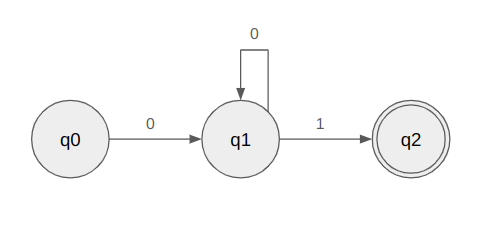
\includegraphics[width=0.9\textwidth]{images/pl/auto1.png}
    \caption{Autómata finito determinista para reconocimiento de la expresión regular $0^+1$.}
    \label{fig:PLAutomt}
\end{figure}

\subsection{Autómatas con pila}\label{subsection:automatPila}
Los autómatas con pila son cruciales para analizar gramáticas independientes del contexto, que generan lenguajes más complejos que los regulares. A diferencia de los autómatas finitos, estos autómatas poseen una pila para almacenar y recuperar información, lo que les permite manejar estructuras anidadas y dependencias a largo plazo.

Formalmente, un autómata con pila se define como una séptupla que incluye un conjunto de estados, un alfabeto de entrada, un alfabeto de pila, una función de transición, un estado inicial, un símbolo inicial de pila y un conjunto de estados finales. Existen versiones deterministas y no deterministas, siendo los deterministas aquellos que aceptan una cadena si, al finalizar su procesamiento, llegan a un estado final con la pila vacía. Esto garantiza que el autómata no solo reconozca la secuencia de símbolos de la entrada, sino que también cumpla con las estructuras de los lenguajes independientes del contexto.

\noindent
He aquí la escritura formal de un autómata con pila:
\begin{align*}
    M = (Q,A,B,\delta,q_0,Z_0,F)
\end{align*}

\noindent
donde:
\begin{itemize}
    \item $Q$ es un conjunto finito llamado \textbf{conjunto de estados}.
    \item $A$ es un alfabeto llamado \textbf{alfabeto de entrada}.
    \item $B$ es un alfabeto llamado \textbf{alfabeto de pila}.
    \item $\delta$ es una aplicación llamada \textbf{función de transición}.
    \item $q_0$ es un elemento de $Q$ llamado \textbf{estado inicial}.
    \item $Z_0 \in B$ es el \textbf{símbolo inicial de pila}
    \item $F$ es un subconjunto de $Q$, llamado \textbf{conjunto de estados finales}.
\end{itemize}

\section{Herramientas de procesamiento de lenguajes. Compiladores e intérpretes}\label{section:compiladores}
Lo acontecido en secciones anteriores en este capítulo ofrecen un marco teórico más que suficiente para el desarrollo de los siguientes capítulos que se centran en la parte práctica del proyecto. En esta última sección se hablará de herramientas prácticas para el procesamiento de lenguajes: los \textit{compiladores} e \textit{intérpretes}. Estas herramientas tienen como objetivo convertir el código fuente escrito en un lenguaje de programación a un formático que la máquina pueda ejecutar o interpretar directamente.

Un \textbf{compilador} es un programa que traduce código fuente escrito en lenguaje de alto nivel a lenguaje máquina o a un código intermedio. El proceso de compilación consta de varias fases:

\begin{enumerate}
    \item \textbf{Análisis léxico}: 
        \begin{itemize}
            \item El compilador lee el código fuente y lo descompone en tokens.
            \item Los tokens pueden ser identificadores, palabras clave, constantes, operadores, etc.
            \item Se simplifica y estructura el código fuente para las fases posteriores.
        \end{itemize}

    \item \textbf{Análisis sintáctico}:
        \begin{itemize}
            \item Organiza los tokens en un árbol sintáctico que representa la estructura gramatical.
            \item Verifica que la secuencia de tokens siga las reglas gramaticales del lenguaje.
            \item Identifica errores de sintaxis como paréntesis faltantes o errores en construcciones de bucles.
        \end{itemize}

    \item \textbf{Análisis semántico}:
        \begin{itemize}
            \item Verifica la corrección semántica del código, asegurando que los elementos del programa tengan sentido en su contexto.
            \item Incluye la verificación de tipos de datos y la coherencia en el uso de variables y funciones.
            \item Detecta errores como asignaciones de tipos de datos incorrectos o llamadas incorrectas a funciones.
        \end{itemize}

    \item \textbf{Generación de código intermedio}:
        \begin{itemize}
            \item Transforma el árbol sintáctico en una representación intermedia.
            \item Esta representación es independiente del lenguaje de programación y del hardware.
            \item Facilita la optimización del código y prepara la generación del código máquina.
        \end{itemize}

    \item \textbf{Optimización de código}:
        \begin{itemize}
            \item Mejora la representación intermedia para aumentar la eficiencia del programa.
            \item Incluye la eliminación de código inaccesible y la optimización de bucles.
            \item Esencial para mejorar el rendimiento y la eficiencia del código compilado.
        \end{itemize}

    \item \textbf{Generación de código máquina}:
        \begin{itemize}
            \item Convierte la representación intermedia en código de máquina ejecutable por el procesador.
            \item El código generado está optimizado para el hardware específico de destino.
            \item Completa el proceso de traducción resultando en un programa ejecutable o archivo objeto.
        \end{itemize}
\end{enumerate}


A diferencia de los compiladores, un \textbf{intérprete} no genera un archivo de salida ejecutable. En su lugar, leen y ejecutan el código fuente directamente, traduciendo el programa a medida que se ejecuta. Esto permite una mayor flexibilidad y una iteración más rápida durante el desarrollo, aunque puede tener un rendimiento más lento en comparación con los programas compilados. Los intérpretes también utilizan técnicas de análisis léxico y sintáctico para entender el código fuente, pero ejecutan las instrucciones inmediatamente después de su análisis.

También hay una variante que combina ambos enfoques, que es lo que se denomina como \textbf{compilador en tiempo de ejecución} (o \textit{Just-In-Time}). En la práctica en este proyecto, aunque se dispone de una fase de compilación que traduce código del lenguaje a código intermedio, su funcionamiento es más semejante al de un \textit{intérprete}, al traducir inmediatamente dichas instrucciones intermedias.

\begin{figure}[h]
    \centering
    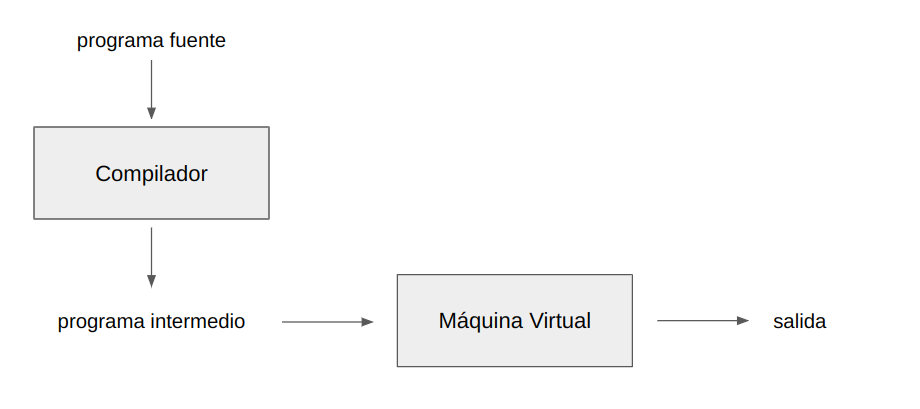
\includegraphics[width=1.0\textwidth]{images/pl/jit.png}
    \caption{Esquema de un compilador en tiempo de ejecución.}
    \label{fig:JITCompiler}
\end{figure}